\documentclass[border=10pt]{standalone}

\usepackage{tikz}
\usepackage{tikzsymbols}
\usetikzlibrary{calc,patterns,shapes.geometric}

\def\centerarc[#1](#2)(#3:#4:#5){\draw[#1] ($(#2)+({#5*cos(#3)},{#5*sin(#3)})$) arc (#3:#4:#5);}

\begin{document}
	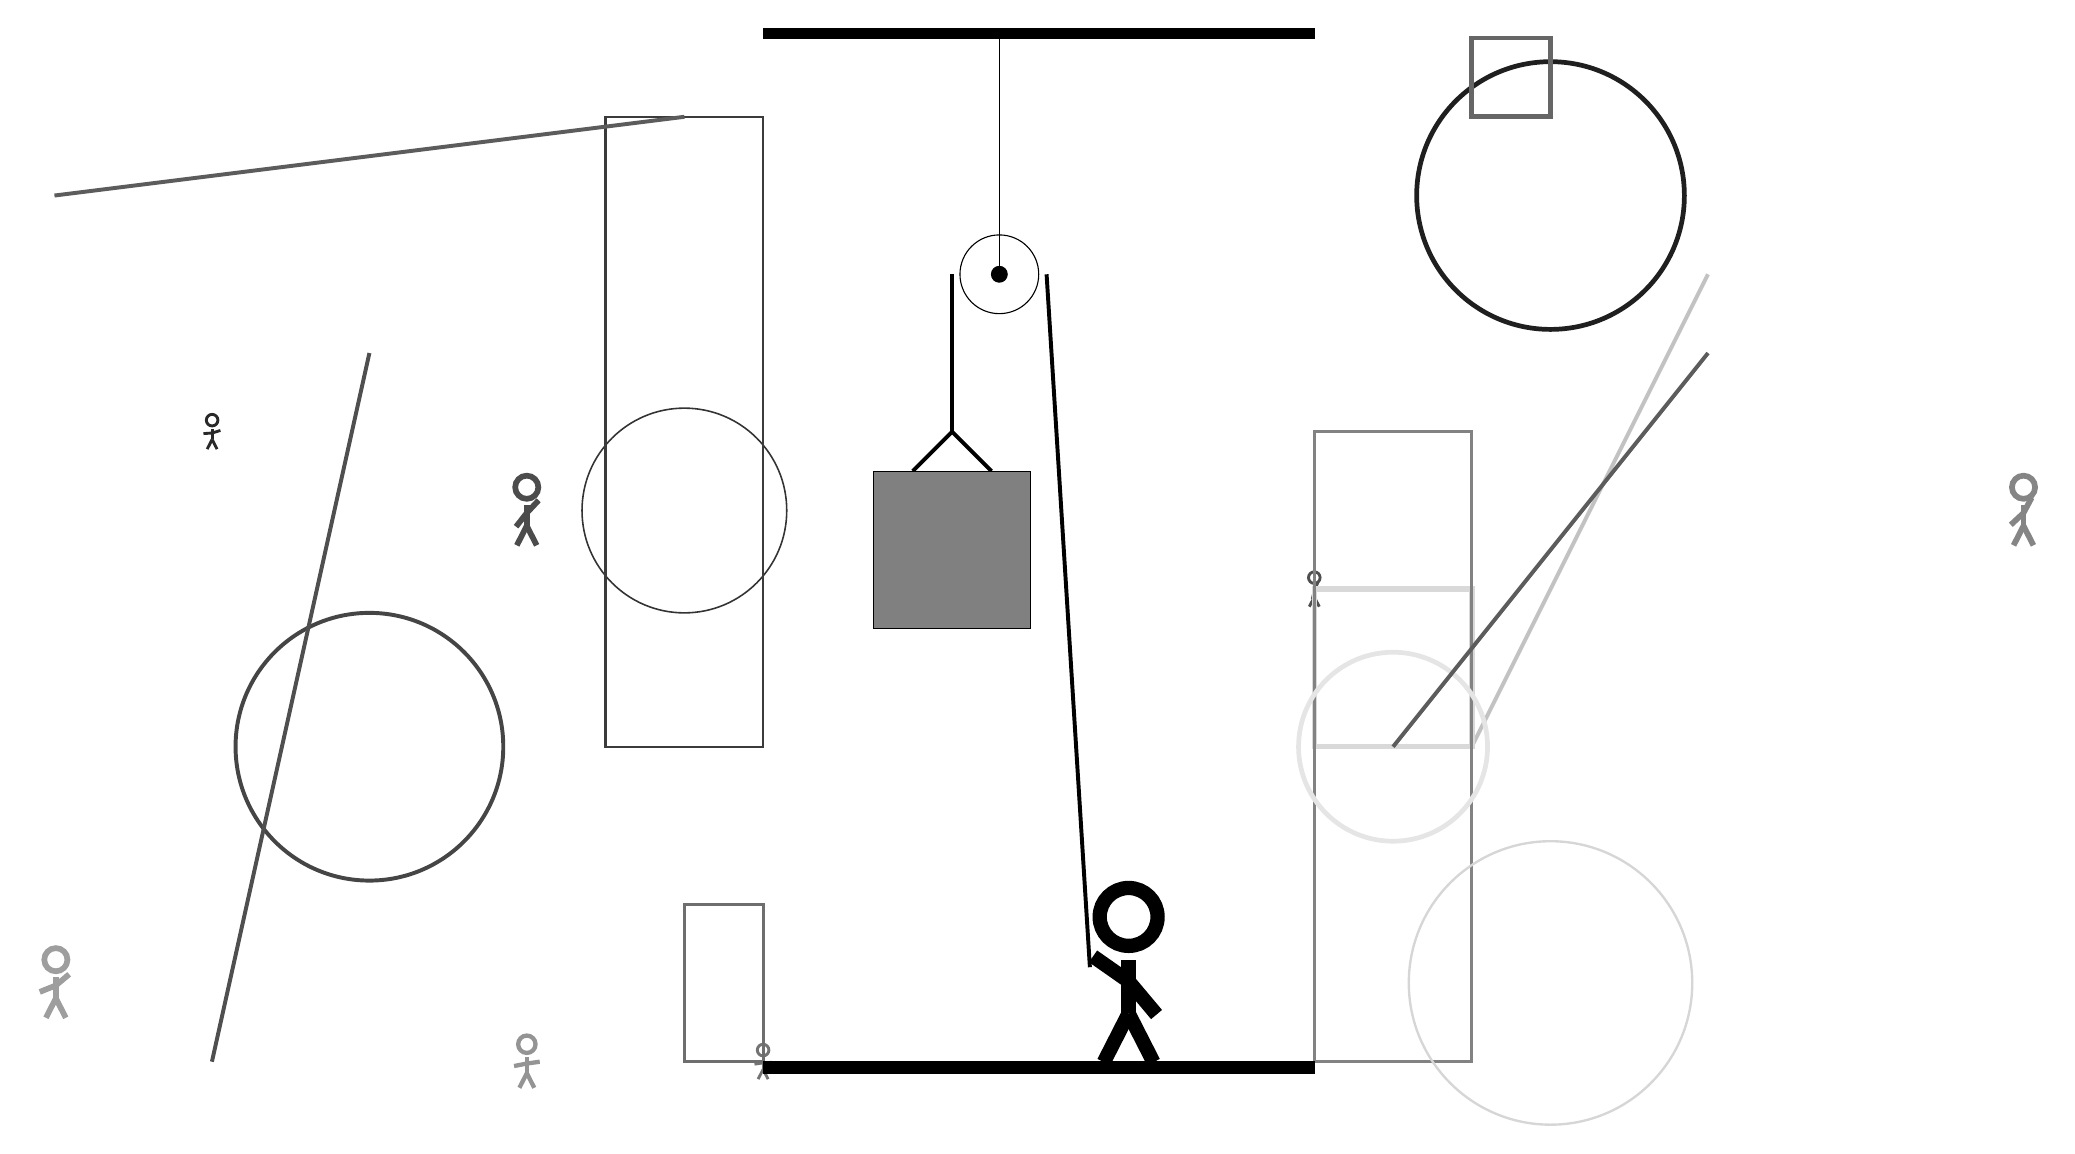
\begin{tikzpicture}
		%%%%% START %%%%%
		
		\draw[fill=black] (-2, 10) rectangle (5, 10.125);
		
		\node[line width=0.2mm, color=black!55] at (-2, -3) {\Strichmaxerl[2][8][4]};
		
		\node[line width=0.5mm, color=black!38] at (-11, -2) {\Strichmaxerl[4][22][40]};
		\node[line width=0.6mm, color=black!69] at (5, 3) {\Strichmaxerl[2][77][66]};
		\draw[line width=0.5mm, color=black!24](10, 7) -- (7, 1);
		\draw[line width=0.7mm, color=black!15] (5, 1) rectangle (7, 3);
		
		\node[line width=0.4mm, color=black!70] at (-5, 4) {\Strichmaxerl[4][52][47]};
		
		\draw [line width=0.5mm, color=black!73](-7, 1) circle (1.7);
		
		\draw[line width=0.4mm, color=black!49] (7, -3) rectangle (5, 5);
		\draw [line width=0.6mm, color=black!88](8, 8) circle (1.7);
		
		\node[line width=0.5mm, color=black!84] at (-9, 5) {\Strichmaxerl[2][4][17]};
		
		\draw [line width=0.2mm, color=black!80](-3, 4) circle (1.3);
		\draw[line width=0.5mm, color=black!69](-7, 6) -- (-9, -3);
		\draw [line width=0.6mm, color=black!10](6, 1) circle (1.2);
		\draw[line width=0.4mm, color=black!57] (-3, -3) rectangle (-2, -1);
		\draw[line width=0.3mm, color=black!77] (-4, 9) rectangle (-2, 1);
		\node[line width=0.3mm, color=black!48] at (14, 4) {\Strichmaxerl[4][43][62]};
		\draw[line width=0.5mm, color=black!64](-3, 9) -- (-11, 8);
		
		\node[line width=0.2mm, color=black!42] at (-5, -3) {\Strichmaxerl[3][11][8]};
		\draw[line width=0.5mm, color=black!64](6, 1) -- (10, 6);
		
		\draw [line width=0.3mm, color=black!16](8, -2) circle (1.8);
		\draw[line width=0.6mm, color=black!60] (7, 9) rectangle (8, 10);
		
		
		\draw (1, 7) circle (0.5);
		\draw[fill=black] (1, 7) circle (0.1);
		\draw (1, 10) -- (1, 7);
		
		\draw[line width=0.5mm] (-0.1, 4.5) -- (0.4, 5.0) -- (0.9, 4.5);
		\draw[fill=black!50] (-0.6, 4.5) rectangle (1.4, 2.5);
		
		\draw[line width=0.5mm] (0.4, 7) -- (0.4, 5.0);
		\centerarc[line width=0.5mm](1, 7)(0:180:0.6);
		\draw[line width=0.5mm](1.6, 7) -- (2.15, -1.8);
		
		\node at (2.6, -1.9) {\Strichmaxerl[10][-35][-50]};
		
		\draw[fill=black] (-2, -3) rectangle (5, -3.15);
		
		%%%%% END %%%%%
	\end{tikzpicture}
\end{document}